\documentclass[11pt,a4paper,DIV=9]{scrartcl}

\usepackage{pgf}
\usepackage{tikz}
\usetikzlibrary{arrows,automata,positioning,shadows}
\usepackage{ngerman}
\usepackage[utf8]{inputenc}
\usepackage{amsmath,amssymb}
\usetikzlibrary{shapes,snakes}
% Schriftart ändern
\renewcommand{\rmdefault}{ppl}
%Möglichkeit zur Änderung von Überschriften
\usepackage{sectsty}
%Überschrift \section uandern
\definecolor{blue}{RGB}{76 , 92, 153}
\allsectionsfont{\color{blue}}
\paragraphfont{\color{blue}}

%Variable Blattnummer
\newcommand{\blatt}[1]{
  \newcommand{\blattnr}{#1}
}
%Aufgabe und Aufgabenteil definieren
\newcounter{temp}
\newcommand{\aufgabe}[1]{
  \setcounter{temp}{\value{subsection}}
  \setcounter{subsection}{#1}
  \addtocounter{subsection}{-1}
  \subsection{Aufgabe}
  \setcounter{subsection}{\value{temp}}
}
\newcommand{\teil}[2][]{
  \subsubsection*{#2) #1}
}
\renewcommand{\author}[1]{\renewcommand{\author}{#1}}
\renewcommand{\title}[1]{\renewcommand{\title}{#1}}
\newcommand{\makehomeworktitle}{
  \begin{minipage}[t]{6.5cm}
    \sf{\author}
  \end{minipage}
  \begin{minipage}[t]{6.5cm}
    \begin{flushright}
      \sf{\title\\\today}
    \end{flushright}
  \end{minipage}
  \\[0.2cm]
  \begin{center}
    \sf{
      \color{blue}{
        \LARGE{Dokumentation First.FM}
      }
    }
  \end{center}
  \vspace{0.1cm}
}

%%%%%%%%%%%%%%%%%%%%%%%%
%%% Statisch
\author{{[}4131658{]} Jan Germann \\{[}4054962{]} Christian Ratz\\Übungsgruppe 1}
\title{SQL Praktikum}

%%% Auf jedes Hausaufgabenblatt anpassen
\blatt{1}
%%%%%%%%%%%%%%%%%%%%%%%%
\begin{document}
\makehomeworktitle
\tableofcontents
\newpage
\section{Einleitung}
  \subsection{Allgemeines}
    In dieser Dokumentation werden die Besonderheiten des Klassendiagramms, für das communitybasierte Musik-Streamingportal \textsc{first.fm}, erläutert. Bei dem Musik-Streamingportal \textsc{first.fm}, haben Benutzer die Möglichkeit selbstkomponierte Musik zu veröffentlichen, Musik anderer Benutzer oder Bands zu hören sowie selbst einer Band beizutreten (haben Sie wirklich die M\"oglichkeit einer Band beizutreten?).\\
    Am Ende dieser Dokumentation ist, zur besseren Übersicht, das komplette Klassendiagramm noch einmal in seiner Vollständigkeit zu finden.

  \subsection{Formatierung} 
    In der Dokumentation sowie im dazugehörigen Diagramm gilt die folgende Formatierung.

    \begin{description}
      \item [Klassennamen] \hfill \\
        Der Name einer Klasse ist im Regelfall \textbf{fett} formatiert.
      \item [Attribute] \hfill \\
        Attribute einer Klasse sind folgendermaßen gekennzeichnet
        \begin{itemize}
          \item[-] Reguläres Attribut
          \item[*] Attribut ist Teil des Primärschlüssel
          \item[/] Abgeleitetes Attribut
          \item[+] Fremdschlüssel
        \end{itemize}
      \item[Relationentypen] \hfill
      \begin{itemize}
        \item Reguläre Relationen zwischen Klassen sind durch eine einfache schwarze Linie gekennzeichnet.
        \item Sogenannte \textit{XOR}-Relationen besitzen an der ausgehenden Klasse ein Rautesymbol ($\blacklozenge$). Hierbei darf die Klasse, für die gespeicherte Entität, nur mit einer einzigen der Klassen gleichzeitig in Relation stehen.
      \end{itemize}
    \end{description}

\section{Klassen}
  \subsection{User}
    Eine Entität der Klasse \textbf{User} wird aus Speicherplatzgründen durch einen Surrogatschlüssel (*id) identifiziert. Ein anderer Schlüsselkandidat ist hierbei der -loginname, dieser ist ebenfalls einmalig. Als weitere Besonderheit ist hierbei das Attribut -online zu sehen, welches \texttt{wahr} ist wenn der Benutzer online ist und sonst \texttt{falsch}. Der Onlinestatus lässt sich leider nicht ohne Weiteres aus dem Attribut -last\_seen ableiten. Ein User ist nach dem Abmelden sofort Offline, allerdings auch sobald die Differenz zwischen -last\_seen und der Jetztzeit größer als 15 Minuten ist.
  \subsection{Band}
    Eine \textbf{Band} besteht aus mindestens einem User. Dies mag auf Anhieb nicht sinnvoll erscheinen, allerdings kann ein Benutzer auch Mitglied einer Band sein, ohne dass der Rest der Band bei \textsc{first.fm} einen Account haben muss. 
  \subsection{Bandmember}
    Die Klasse \textbf{Bandmember} soll es den Benutzern einer Band ermöglichen, Mitglieder einer Band hinzuzufügen welche nicht über einen Benutzeraccount bei \textsc{first.fm} verfügen. Um die Zugehörigkeit zu einer bestimmten Band zu definieren verfügen diese Entitäten über den Fremdschlüssel +band\_id. Desweiteren verfügen diese Entitäten über den Fremdschlüssel +instrument\_id, welche das von Ihnen in der Band gespielte Instrument definiert.
  \subsection{Song}
    Ein einzelner Song verfügt natürlich immer über einen Titel (-title) und wurde meist zu einem bestimmten Datum veröffentlicht (-release\_date). Ausserdem verfügt die Klasse \textbf{Song} noch über ein abgeleitetes Attribut -/status welches sich aus der Quantität und Qualität von Bewertungen aus der Tabelle \textbf{Songrating} ableitet. (Bei einer Bewertung von 4,5 bei \"uber 10000 Bewertungen erh\"alt der Song einer Goldstatus, bei einer Bewertung von 4,6 bei \"uber 100000 Bewertungen den Platinstatus.) 
  \subsection{Album}
    Hier wird dargestellt, welchen Namen (-name) das Album tr\"agt, an welchem Datum (-date) es ver\"offentlicht wurde und welchem Label (+label\_id) es zugeordnet wird.
  \subsection{Album2Genre}
    Relationentabelle zwischen einem Album und einem oder mehreren Genres. Ist notwendig um anzugeben, welchem Genre oder welchen Genres das Album angeh\"ort.
  \subsection{Label}
    Die Klasse \textbf{Label} ist eine Liste von Labels, welche Alben veröffentlicht haben.
  \subsection{Genre}
    Die Klasse \textbf{Genre} ist eine Liste von Genre denen einzelne Songs oder ganze Alben angehören können. Der -name ist hierbei verpflichtend.
  \subsection{Comment}
    Die Klasse \textbf{Comment} ist n\"otig f\"ur das Erstellen von Kommentaren zu Songs, Alben, Bands oder Solok\"unstlern. Hierbei wird sowohl eine Zeit (-timestamp) an der das Kommentar erstellt wurde als auch der Inhalt (-content) des Kommentars und der Name des Benutzers (+user\_id) der den Kommentar (*id) erstellt hat, gespeichert.
  \subsection{Comment2User}
    Relationentabelle zwischen einem Kommentar und einem Benutzer. Damit ein Benutzer einen anderen Benutzer oder Solok\"unstler kommentieren kann.
  \subsection{Comment2Song}
    Relationentabelle zwischen einem Kommentar und einem Song. Notwendig damit Benutzer Songs kommentieren k\"onnen.
  \subsection{Comment2Band}
    Relationentabelle zwischen einem Kommentar und einer Band. Ist dazu da, dass Benutzer ebenso Kommentare zu Bands abgeben k\"onnen.
  \subsection{Instrument}
    Die Klasse \textbf{Instrument} ist Liste von Instrumenten, welche von Benutzern oder Bandmitgliedern gespielt werden.
  \subsection{Upload}
    Relationentabelle zwischen einem Benutzer und einem Song. Diese Tabelle ist n\"otig um zu kennzeichnen welcher Benutzer einen bestimmten Song zu einem bestimmten Datum hochgeladen hat.
  \subsection{Recommendation}
    Diese Tabelle soll es einem Benutzer (+*recommender\_id) ermöglicht, einem anderen Benutzer (+*recipient\_id) einen bestimmten Song (+*song\_id) zu empfehlen.
  \subsection{Songrating}
   Relationentabelle zwischen einem Benutzer und einem Song. Ist notwendig, damit ein bestimmter Benutzer (+*user\_id) zu einem oder zu mehreren bestimmten Songs (+*song\_id) auf einer Skala von eins bis f\"unf Bewertungen (-rating) abgeben kann. Aus der Bewertung eines Songs leitet sich dann das Attribut -/status der Klasse \textbf{User} ab.
  \subsection{Friendslist}
    Diese Tabelle stellt die Freundschaftsbeziehungen zwischen Benutzern dar. Eine Freundschaft ist immer zweiseitig und somit wird gezeigt, dass ein Benutzer (+*user\_id) mit einem anderen Benutzer (+*friend\_id) in einem freundschaftlichem Verhältnis steht. Da es sein kann, dass ein Benutzer nicht mit einem anderen befreundet sein möchte, gibt es noch das Attribut -active welches nur dann den Wert \texttt{wahr} besitzt wenn die Freundschaft von dem anderen Benutzer bestätigt wurde.
  \subsection{User2Played}
    Relationentabelle zwischen einem Benutzer und einem Song. Es soll dem Benutzer möglich sein herauszufinden wann und damit auch wie oft er einen bestimmten Song schon abgespielt hat.
  \subsection{Artist2Song}
    Relationentabelle zwischen einem Benutzer und einem Song, falls der Song eine Solo-Komposition des Benutzers ist.
  \subsection{User2Band}
    Die Klasse \textbf{User2Band} definiert die Zugehörigkeit eines Benutzers zu einer Band, sowie über den Fremdschlüssel +instrument\_id, der das von dem Benutzer in der Band gespielte Instrument darstellt.
  \subsection{Band2Song}
    Relationentabelle zwischen einer Band und einem Song, falls der Song eine Komposition einer Band ist.
  \subsection{Song2Genre}
    Relationentabelle zwischen mehreren Genres und einem Song. Ermöglicht es einem Song mehrere Genres zuzuordnen.
  \subsection{Song2Album}
    Relationentabelle zwischen einem Album und einem Song, falls der Song Teil eines Albums oder mehrerer Alben ist.



\section{Klassendiagramm}
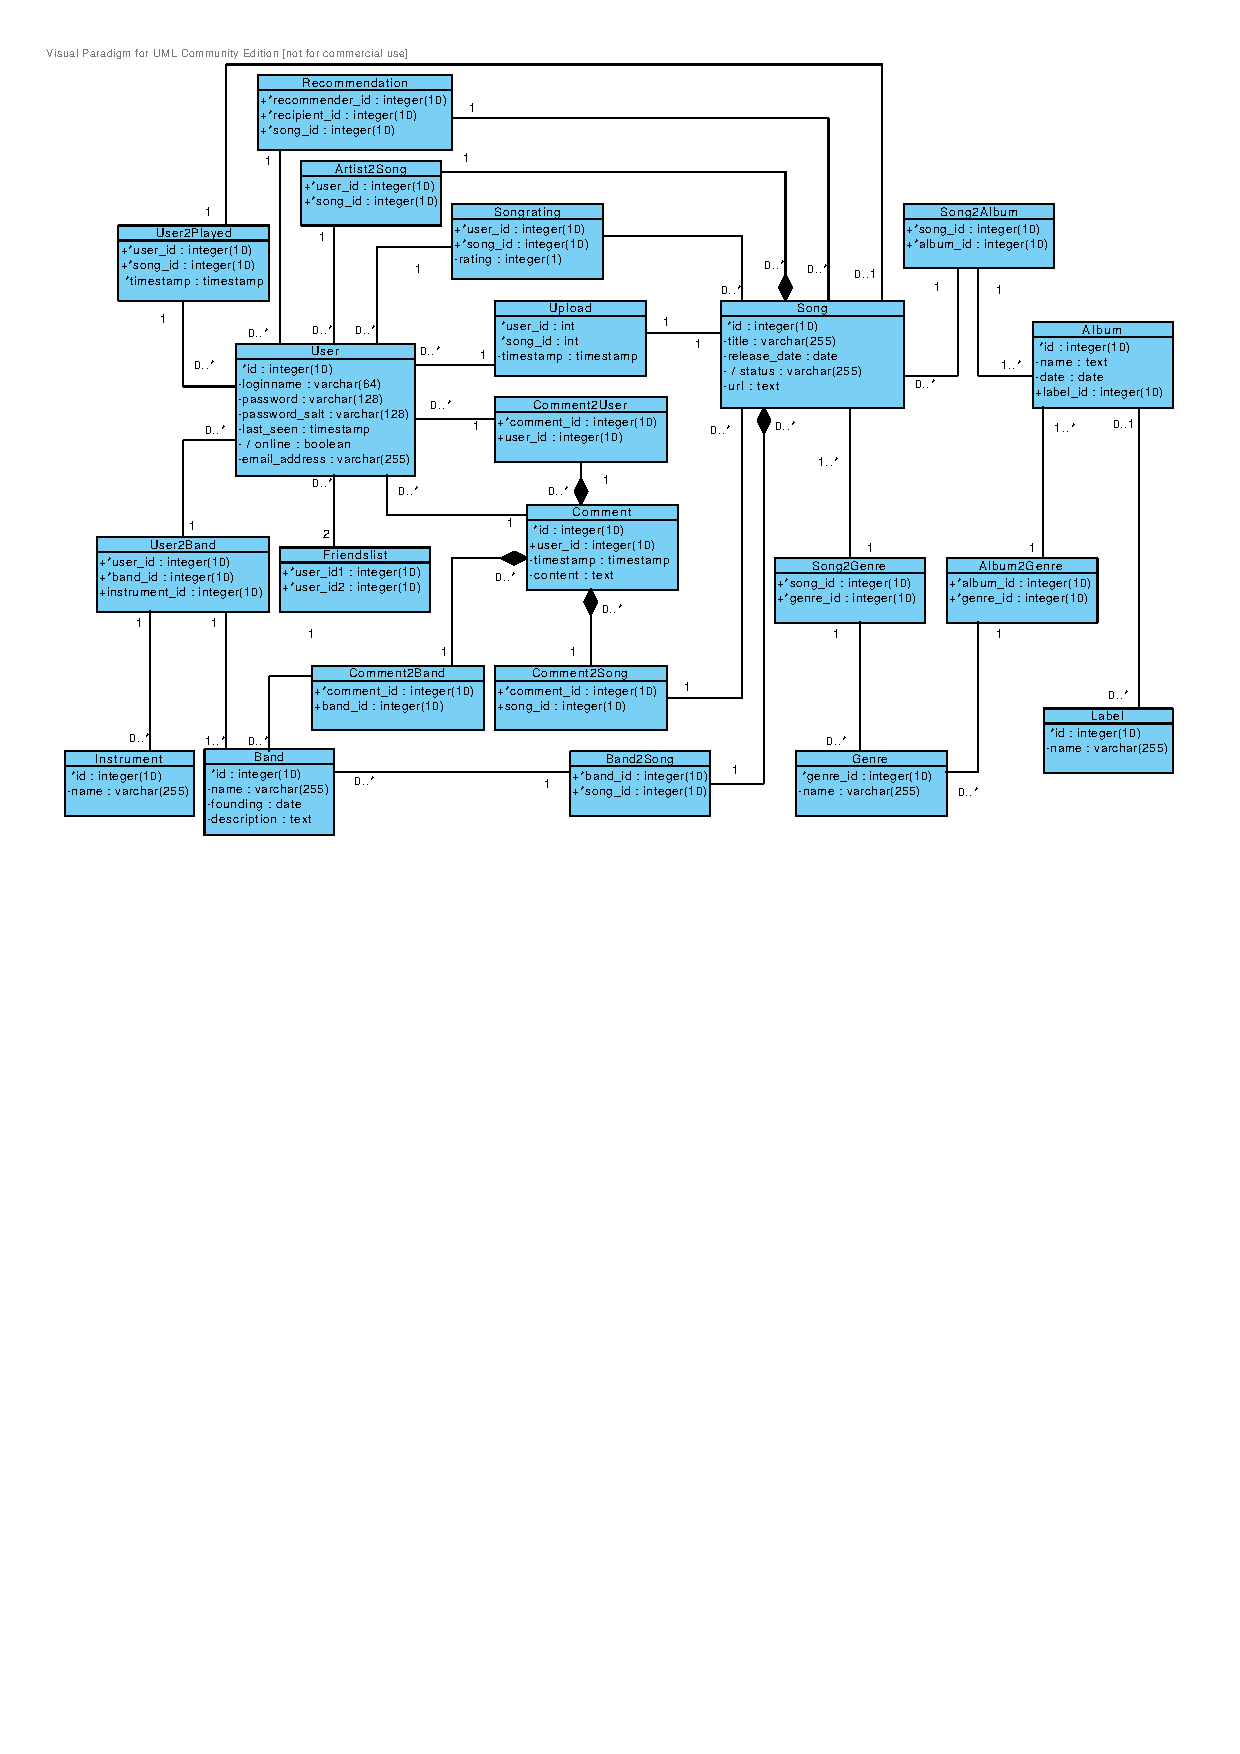
\includegraphics[page=1, angle=90,trim=0cm 0cm 1.1cm 1cm, clip=true, scale=1.1]{Diagram1}
\end{document}